\documentclass[conference]{IEEEtran}
\usepackage[top=3cm, bottom=2cm, left=2cm, right=2cm, columnsep=20pt]{geometry}
\usepackage{pdfpages}
\usepackage{graphicx}
\usepackage{etoolbox}
\apptocmd{\sloppy}{\hbadness 10000\relax}{}{}
% \usepackage[numbers]{natbib}
\usepackage[T1]{fontenc}
\usepackage{ragged2e}
\usepackage[french]{babel}
\usepackage{listings}
\usepackage{color}
\usepackage{soul}
\usepackage[utf8]{inputenc}
\usepackage[export]{adjustbox}
\usepackage{caption}
\usepackage{mathrsfs, amsmath}
\usepackage{amssymb}
\usepackage{float}
\usepackage{csquotes}
\usepackage{fancyhdr}
\usepackage{wallpaper}
\usepackage{siunitx}
\usepackage[indent]{parskip}
\usepackage{textcomp}
\usepackage{gensymb}
\usepackage{multirow}
\usepackage[hidelinks]{hyperref}
\usepackage{abstract}
\usepackage{subcaption}
\usepackage{tabularx}
\usepackage{biblatex}
\addbibresource{bibliographie.bib}

% \renewcommand{\abstractnamefont}{\normalfont\bfseries}
% \renewcommand{\abstracttextfont}{\normalfont\itshape}
\usepackage{titlesec}
% \titleformat{\section}{\large\bfseries}{\thesection}{1em}{}
% \titleformat{\subsection}{\normalsize\bfseries}{\thesubsection}{1em}{}
% \titleformat{\subsubsection}{\normalsize\bfseries}{\thesubsubsection}{1em}{}

\usepackage{xcolor}
\definecolor{codegreen}{rgb}{0,0.6,0}
\definecolor{codegray}{rgb}{0.5,0.5,0.5}
\definecolor{codepurple}{rgb}{0.58,0,0.82}
\definecolor{backcolour}{rgb}{0.95,0.95,0.92}
\lstdefinestyle{mystyle}{
    backgroundcolor=\color{backcolour},   
    commentstyle=\color{codegreen},
    keywordstyle=\color{magenta},
    numberstyle=\tiny\color{codegray},
    stringstyle=\color{codepurple},
    basicstyle=\ttfamily\footnotesize,
    breakatwhitespace=false,         
    breaklines=true,                 
    captionpos=b,                    
    keepspaces=true,                 
    numbers=left,                    
    numbersep=5pt,                  
    showspaces=false,                
    showstringspaces=false,
    showtabs=false,                  
    tabsize=2
}
\lstset{style=mystyle}

\usepackage[most]{tcolorbox}
\newtcolorbox{note}[1][]{
  enhanced jigsaw,
  borderline west={2pt}{0pt}{black},
  sharp corners,
  boxrule=0pt, 
  fonttitle={\large\bfseries},
  coltitle={black},
  title={Note:\ },
  attach title to upper,
  #1
}

\pagestyle{plain}
%----------------------------------------------------

\setlength{\parindent}{0pt}
\DeclareCaptionLabelFormat{mycaptionlabel}{#1 #2}
\captionsetup[figure]{labelsep=colon}
\captionsetup{labelformat=mycaptionlabel}
\captionsetup[figure]{name={Figure }}
\captionsetup[table]{name=Tableau}
\newcolumntype{Y}[1]{>{\Centering\hspace{0pt}\hsize=#1\hsize}X}
\newcommand{\inlinecode}{\normalfont\texttt}
\usepackage{enumitem}
\setlist[itemize]{label=\textbullet}

\begin{document}

%----------------------------------------------------
\title{Microscope\\
\large Travail préparatoire \\
PHS3910 -- Techniques expérimentales et instrumentation\\ 
Équipe L3}

\author{\IEEEauthorblockN{Émile Guertin-Picard}
\IEEEauthorblockA{2208363}
\and
\IEEEauthorblockN{Maxime Rouillon}
\IEEEauthorblockA{2213291}
\and
\IEEEauthorblockN{Marie-Lou Dessureault}
\IEEEauthorblockA{2211129}
\and
\IEEEauthorblockN{Philippine Beaubois}
\IEEEauthorblockA{2211153}
}

\maketitle

\textit{\textbf{Résumé} -- yap yap}

\section{Introduction}


\textcolor{red}{yap yap}


\section{Méthodes \label{methodes}}

\textcolor{red}{yap yap}

\begin{figure}[H]
  \centering
  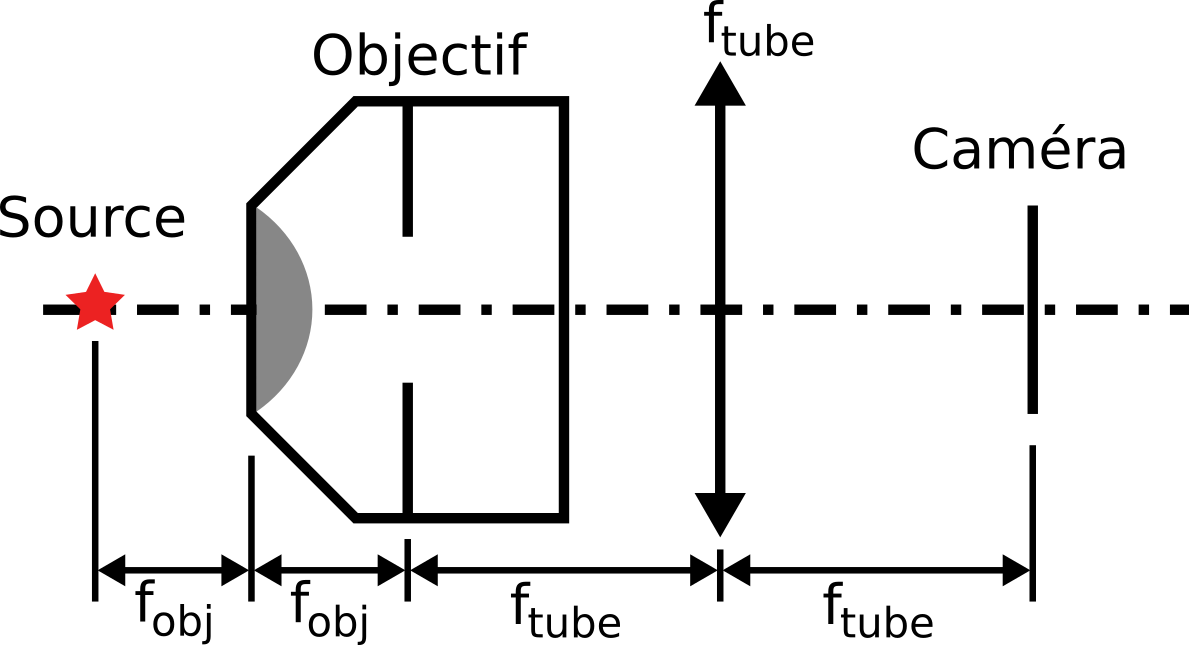
\includegraphics[scale=2.3]{systeme.png}
  \caption{Système optique de microscope.}
  \label{sys}
\end{figure}



\textcolor{red}{yap yap}

Afin de déterminer quels objectifs de microscope considérer pour le produit final, la définition
de la résolution est nécessaire pour la vérification du théorème d'échantillonage de Nyquist. Soit $d$,
la limite de diffraction pour une source ponctuelle au travers d'une ouverture \textcolor{red}{source video}:
\begin{equation}
  d = \frac{\lambda}{2 \text{NA}},
\end{equation}

où $\lambda$ est la longueur d'onde éclairant l'échantillon observé et NA est l'ouverture numérique de
l'objectif. Cette limite de diffraction est la résolution du système. Ainsi, selon le théorème
de Nyquist, la taille effective d'un pixel de la caméra $P$ dans le plan de l'objet observé doit respecter :

\begin{equation}\label{nyquist}
  P \leq \frac{d}{2} = \frac{\lambda}{4 \text{NA} }.
\end{equation}

Le calcul de cette taille $P$ est obtenue à partir du grossissement $M$ de l'objectif ainsi qu'avec la
focale de la lentille de tube $f_{tube}$. Le grossissement est défini tel que :

\begin{equation}
  M = \frac{f_{tube}}{f_{obj}},
\end{equation}

où $f_{obj}$ est la longueur focale de la lentille objectif. Le grossissement $M$ connu des lentilles suit
un standard de la \textit{Royal Microscopical Society} (RMS) qui pose $f_{tube}$ à 160 mm
\textcolor{red}{source A}. Ainsi, pour avoir le grossissement réel $M_{r}$, il faut convertir avec la 
formule suivante :

% Source A : https://www.microscopyu.com/microscopy-basics/infinity-optical-systems

\begin{equation}
  f_{1}= \frac{160 \text{ mm} }{M} \Rightarrow M_{r} = \frac{f_{obj}M}{160 \text{ mm} }.
\end{equation}

La taille réelle d'un pixel de caméra $p_r$, d'une valeur de 3.45 µm pour la caméra Zelux CS165MU
mise à disposition pour ce contrat \textcolor{red}{source B}, peut être convertie en taille effective
avec le grossissement réel :

\begin{equation}
  P = \frac{p_{r}}{M_{r}} = \frac{p_{r}\;160 \text{ mm}}{f_{obj}M}.
\end{equation}

Ainsi, pour un système avec $f_{obj}$ et $M$ connus, il est possible de déterminer si le théorème 
(\ref{nyquist}) est respecté pour une longueur d'onde donnée. Cela a permis de déterminer quelles 
combinaisons de lentille tube, d'objectif de microscope et de source de lumière qui ne sont pas 
sujettes au phénomène d'\textit{aliasing}, conséquence du non respect de Nyquist où l'information
réelle sur l'image est perdue.

% source B : https://www.thorlabs.com/thorproduct.cfm?partnumber=CS165MU

\section{Résultats \label{resultats}}



\section{Discussion}

\textcolor{red}{quel combo a la meilleure resolution $d$ avec le moins d'incertitude}

%\printbibliography

\clearpage

\section{Annexes}

\subsection{Preuve de correction par Antidote}

\clearpage


\end{document}
